\documentclass[12pt, border=12pt]{standalone}
\usepackage[utf8]{inputenc}
\usepackage[utf8]{vietnam}
\usepackage{amsmath,amsfonts,amssymb}
\usepackage{type1cm}
\usepackage{graphicx}
\usepackage{multirow}
\usepackage{multicol}
\usepackage{array}
\usepackage{comment}
\usepackage[unicode]{hyperref}
\usepackage{tikz}
\usepackage{color}
\usepackage[american,cuteinductors,smartlabels]{circuitikz}
\usetikzlibrary{arrows}
\usepackage{tikz}
\usetikzlibrary{calc,patterns,angles,quotes}
\usetikzlibrary{arrows, decorations.markings, calc, fadings, decorations.pathreplacing, patterns, decorations.pathmorphing, positioning}	
%\tikzstyle{every path}=[line width=1.2pt]

\tikzset{middlearrow/.style={
        decoration={markings,
            mark= at position 0.5 with {\arrow{#1}} ,
        },
        postaction={decorate}
    }
}
\begin{document}
	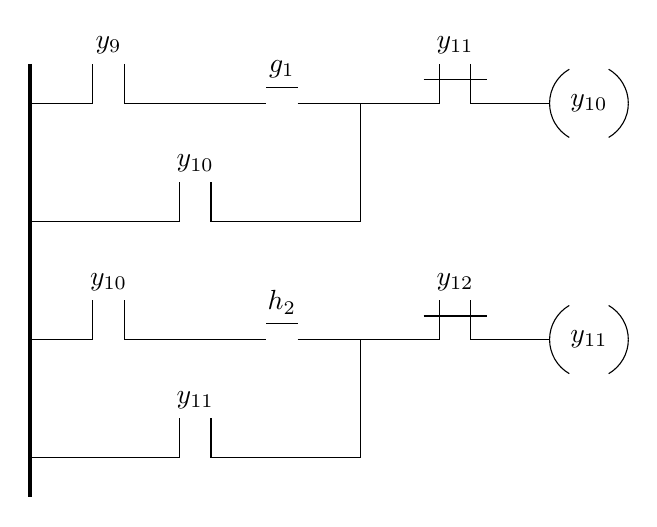
\begin{tikzpicture}[>=triangle 45]
		\draw[ultra thick] (8.5,-5.5) -- (8.5,-11);
						
		\draw (8.5,-6) -- (9.3,-6) -- (9.3,-5.5); \draw (9.7,-5.5) -- (9.7,-6) -- (11.5,-6); \draw (9.5,-5.5) node[above]{$y_9$};  \draw (11.5,-5.8) -- (11.9,-5.8); \draw(11.7,-5.8) node[above]{$g_1$}; \draw (11.9,-6) -- (12.7,-6); \draw (12.7,-6) -- (13.7,-6)-- (13.7,-5.5); \draw (14.1,-5.5) -- (14.1,-6) -- (15.1,-6); \draw (13.5,-5.7) -- (14.3, -5.7); \draw (13.9,-5.5) node[above]{$y_{11}$}; \draw (15.1,-6) arc (180:120:.5);\draw (15.1,-6) arc (180:240:.5); \draw (16.1,-6) arc (0:60:.5);\draw (16.1,-6) arc (0:-60:.5); \draw (15.6,-6) node{$y_{10}$}; \draw (8.5,-7.5) -- (10.4,-7.5) -- (10.4,-7); \draw (10.8,-7) -- (10.8,-7.5)-- (12.7,-7.5) -- (12.7,-6); \draw (10.6,-7) node[above]{$y_{10}$};
						
		\draw (8.5,-9) -- (9.3,-9) -- (9.3,-8.5); \draw (9.7,-8.5) -- (9.7,-9)-- (11.5,-9); \draw (9.5,-8.5) node[above]{$y_{10}$}; \draw (11.5,-8.8) -- (11.9,-8.8); \draw(11.7,-8.8) node[above]{$h_2$}; \draw (11.9,-9) -- (12.7,-9); \draw (12.7,-9) -- (13.7,-9)-- (13.7,-8.5); \draw (14.1,-8.5) -- (14.1,-9) -- (15.1,-9); \draw (13.5,-8.7) -- (14.3, -8.7); \draw (13.9,-8.5) node[above]{$y_{12}$}; \draw (15.1,-9) arc (180:120:.5);\draw (15.1,-9) arc (180:240:.5); \draw (16.1,-9) arc (0:60:.5);\draw (16.1,-9) arc (0:-60:.5); \draw (15.6,-9) node{$y_{11}$}; \draw (8.5,-10.5) -- (10.4,-10.5) -- (10.4,-10); \draw (10.8,-10) -- (10.8,-10.5) -- (12.7,-10.5) -- (12.7,-9); \draw (10.6,-10) node[above]{$y_{11}$};
	\end{tikzpicture}
\end{document}